\documentclass[sigconf,nonacm,balance=false]{acmart}
\usepackage{popets}

% No copyright block, venue headers, DOI or ISBN (nonacm + copyright none).
\setcopyright{none}
\settopmatter{printacmref=false, printccs=false, printfolios=true}

\usepackage{enumitem}
\usepackage{tabularx}
\usepackage{array}
\usepackage{multirow}

\setlist{itemsep=2pt, topsep=4pt}
\graphicspath{{figures/}}

\newcommand{\todo}[1]{{\color{magenta}\bfseries [To-do: #1]}}
\newcommand{\fix}[1]{{\color{red}#1}}
\newcommand{\sys}{\textsc{LicenseWise}}

\begin{document}

\title{LicenseWise: Explaining and Verifying Open-Source License Recommendations with LLMs and Natural Language Inference}
\subtitle{ENSF 621 --- Phase 1 Report}

\author{Opeyemi Ajegbomogun}
\affiliation{%
  \institution{University of Calgary}
  \department{Department of Electrical and Software Engineering}
  \city{Calgary}
  \country{Canada}}

\author{Okemawo Obadofin}
\affiliation{%
  \institution{University of Calgary}
  \department{Department of Electrical and Software Engineering}
  \city{Calgary}
  \country{Canada}}

\renewcommand{\shortauthors}{Ajegbomogun and Obadofin}

\begin{abstract}
Developers routinely choose open-source licenses, or inherit them through dependencies, without fully understanding the obligations involved. Large language models (LLMs) can explain legal text in plain language, but they also produce fluent, unsupported statements, which is especially harmful in licensing. We present \sys{}, a two-stage LLM\,+\,NLI pipeline that takes a natural-language project description and/or a dependency manifest, recommends three licenses from a catalogue of 34 OSI-approved software licenses, and explains each recommendation with plain-language claims that cite and quote a specific license clause. An off-the-shelf natural language inference (NLI) model then checks every claim against its cited clause and labels it \emph{verified}, \emph{unverified}, or \emph{contradicted}. Because no legal domain expert was available, we build all ground truth from public, machine-readable sources: choosealicense.com labels and texts, the SPDX license list, and the Software Heritage license dataset. We evaluate recommendation on 104 model-written, round-trip-validated project descriptions covering 70 requirement profiles, and verification on 729 clause--claim pairs, 146 of which were hand-checked by two annotators (Cohen's $\kappa = 0.88$). The recommender (gpt-oss-120b) places a correct license among its top three for 74\% of descriptions, falling to 60\% when only one to three licenses satisfy the requirements. The verifier (DeBERTa-v3-large) reaches 0.82 accuracy with 0.94 precision on \emph{verified}, but confirms only 69\% of true claims, struggling most with copyleft and commercial-use claims. These results suggest that LLMs are useful for interpreting developer intent and explaining licenses, but that license selection itself should be constrained by structured license knowledge.
\end{abstract}


\keywords{open-source licensing, large language models, natural language inference, explainability, software engineering for ML}

\maketitle

\section{Introduction}
\label{s:intro}

Every piece of shared software carries a license: the legal terms that govern how others may use, modify, and redistribute it. Choosing a license is therefore one of the first engineering decisions in an open-source project, and every dependency a project adopts brings its own license terms with it. Prior work shows that developers often make these decisions with little legal training, struggle to interpret license language, and frequently misunderstand obligations such as copyleft or patent grants~\cite{almeida2017developers,wu2024license}. Two failures follow. A license may be a \emph{wrong fit}, failing to protect what the developer actually cares about, for example choosing a permissive license when improvements were meant to stay open. Or it may \emph{conflict} with the license of a dependency, for example releasing an application under proprietary terms while it is built on a strong-copyleft component.

Existing help does not fit the individual project. Decision guides such as choosealicense.com~\cite{choosealicense} offer a few generic paths, do not consider dependencies, and do not explain why a license fits a particular case. License scanners and compliance tools detect licenses after code is written~\cite{german2010ninka,scancode,xu2023lidetector}; they audit rather than recommend. Lawyers are accurate but slow and costly for students, start-ups, and small teams. Large language models (LLMs) appear well suited to the gap: they can map informal goals (``I want companies running it as a service to share their improvements'') to precise license concepts and explain dense legal text in plain language. However, LLMs also produce confident statements that the source text does not support~\cite{ji2023hallucination,maynez2020faithfulness}, and in licensing a confident wrong answer is worse than no answer.

This report describes \sys{}, the system built in Phase~1 of our ENSF~621 project. \sys{} pairs an LLM with an independent verifier. Stage~1 interprets a project description and/or a dependency manifest and recommends three licenses from a catalogue of 34 OSI-approved software licenses. Stage~2 explains each license with short claims, each of which must cite one license clause and quote it verbatim. A natural language inference (NLI) model then checks every claim against its cited clause, and the user sees each claim marked \emph{verified}, \emph{unverified}, or \emph{contradicted}, with the clause one click away.

A central difficulty, raised early by our instructor, is evaluation without a legal domain expert. We address it by decomposing the problem into tasks whose ground truth can be computed or checked from public, curated data: license permission/condition/limitation labels from choosealicense.com, the SPDX license list~\cite{spdx}, and the Software Heritage license dataset~\cite{zacchiroli2022dataset}.

We investigate three research questions:
\begin{description}[leftmargin=1cm, labelwidth=0.8cm, labelsep=0.2cm, font=\normalfont\bfseries]
    \item[RQ1] \textit{Requirement-to-license mapping.} To what extent can an open-weight LLM, conditioned on a curated license catalogue, map natural-language project requirements to open-source licenses that satisfy them, and how does accuracy vary with requirement specificity (the size of the admissible license set)?
    \item[RQ2] \textit{Claim verification.} How reliably can off-the-shelf NLI models verify LLM-generated claims against the license clauses they cite, as measured on human-validated clause--claim pairs?
    \item[RQ3] \textit{Explanation faithfulness.} To what extent are LLM-generated license explanations grounded in the cited license text, in terms of quote fidelity and textual entailment, and how does NLI-based verification change the claims presented to developers compared with an unverified baseline?
\end{description}

\noindent This report makes the following contributions:
\begin{itemize}
    \item \textbf{A working system} (\sys{} v1): a Python pipeline, a command-line interface, and a React web interface that recommend licenses and present clause-cited, verified explanations (Section~\ref{s:eng}).
    \item \textbf{Two expert-free evaluation datasets}: 77 requirement profiles with computed answer keys and 190 validated natural-language descriptions (RQ1), and 729 clause--claim pairs with human-checked labels (RQ2) (Section~\ref{s:method}).
    \item \textbf{An empirical evaluation} of an open-weight LLM recommender and two off-the-shelf NLI verifiers, identifying where each succeeds and fails (Section~\ref{s:results}).
\end{itemize}

\section{Related Work}
\label{s:related}

\paragraph{Understanding and identifying licenses.}
Empirical studies show that developers misunderstand license terms and struggle with license combinations~\cite{almeida2017developers}, and that license usage in practice is complex and error-prone~\cite{wu2024license}. Tools such as Ninka~\cite{german2010ninka} and the ScanCode toolkit~\cite{scancode} identify licenses in source files, and machine-learning approaches detect license exceptions~\cite{vendome2017exceptions}. More recently, LtRecognizer explores NLP- and LLM-based recognition of license terms~\cite{liu2027ltrecognizer}. These works focus on \emph{identifying} what license or term is present; \sys{} instead \emph{recommends} a license for a new project and explains it.

\paragraph{Compatibility and compliance.}
Kapitsaki et al.\ automate license compatibility checking using SPDX metadata~\cite{kapitsaki2017spdx}, and LiDetector detects incompatibilities among the licenses in a project~\cite{xu2023lidetector}. Curated resources such as the OSADL compatibility matrix~\cite{osadl} encode which licenses can be combined. These approaches audit existing code; our Phase~1 system flags dependency constraints at decision time and plans to use such a matrix as ground truth in Phase~2.

\paragraph{License data.}
The SPDX license list~\cite{spdx} standardises license identifiers, choosealicense.com~\cite{choosealicense} publishes machine-readable permission, condition, and limitation labels, and the Software Heritage archive~\cite{dicosmo2017swh} underlies a large dataset of 6.5 million license-file variants with ScanCode detections~\cite{zacchiroli2022dataset}. We use all three: the first two as our knowledge base and ground truth, the third for exploratory analysis and to check how well our scope covers real-world use.

\paragraph{Faithfulness and NLI-based verification.}
Hallucination, generated content not supported by the source, is a well-documented weakness of neural text generation~\cite{ji2023hallucination,maynez2020faithfulness}. NLI models trained on corpora such as MNLI~\cite{williams2018mnli} and ANLI~\cite{nie2020anli} have been used to detect factual inconsistencies between a source and generated text~\cite{laban2022summac,honovich2022true}. Retrieval-augmented generation grounds outputs in retrieved passages~\cite{lewis2020rag}. \sys{} combines these ideas: the explainer must quote a retrieved clause, and an NLI model (DeBERTa-v3~\cite{he2023debertav3}, compared with RoBERTa~\cite{liu2019roberta}) checks each claim against that clause.

\paragraph{Synthetic evaluation data.}
LLMs are increasingly used to generate data, including instructions and test inputs~\cite{wang2023selfinstruct}. We use one LLM to write natural-language project descriptions from structured requirement profiles and a different LLM to validate them, so that the model under test never generates or validates its own test data.

\section{Engineering Components}
\label{s:eng}

\subsection{Software Engineering}
\label{ss:se}

\paragraph{Requirements elicitation.}
Requirements were elicited from three sources: brainstorming within the team (inputs, outputs, and how users can trust the output); instructor feedback on the proposal, which stressed that evaluation must work without a domain expert and that the scope must be explicit; and a peer review by another project group. The peer review raised six points. Three were already covered (command-line commands, prompt templates, legal disclaimer). Two led to new requirements: warnings for operational failures such as API quota limits and low-confidence verification (FR11), and input hardening against malformed files and prompt injection (a security non-functional requirement). One revealed that reviewers still assumed the vector-retrieval design of our proposal, which prompted us to explain the simplified v1 design more clearly (Section~\ref{ss:changes}).

\paragraph{Requirements.}
Figure~\ref{fig:fr} shows how the core functional requirements link together. The system accepts a project description (FR1) and/or a dependency manifest (FR2); looks up each dependency's license (FR3); recommends exactly three licenses from the catalogue (FR4); explains each with plain-language claims that cite a clause (FR5); verifies every claim (FR6); flags conflicting and unknown dependency licenses (FR7); asks clarifying questions when input is vague (FR8); and shows the quoted clause as evidence (FR9). Peer review added a command-line interface (FR10) and operational warnings (FR11). The main non-functional requirements are \emph{faithfulness} (never mark a false claim as verified; target precision $\geq 0.9$), \emph{transparency} (every claim links to its source clause), \emph{safety} (a ``not legal advice'' disclaimer on every result), \emph{cost} (run on a free API tier plus a local verifier), \emph{privacy} (manifests are never stored), \emph{security and robustness} (file type, size, and parsing checks; inputs treated as untrusted), and \emph{reproducibility} (seeded, versioned data and scripts). We prioritised FR1/FR2, FR4, FR5, FR6, and faithfulness as the top five.

\begin{figure*}[tb]
    \centering
    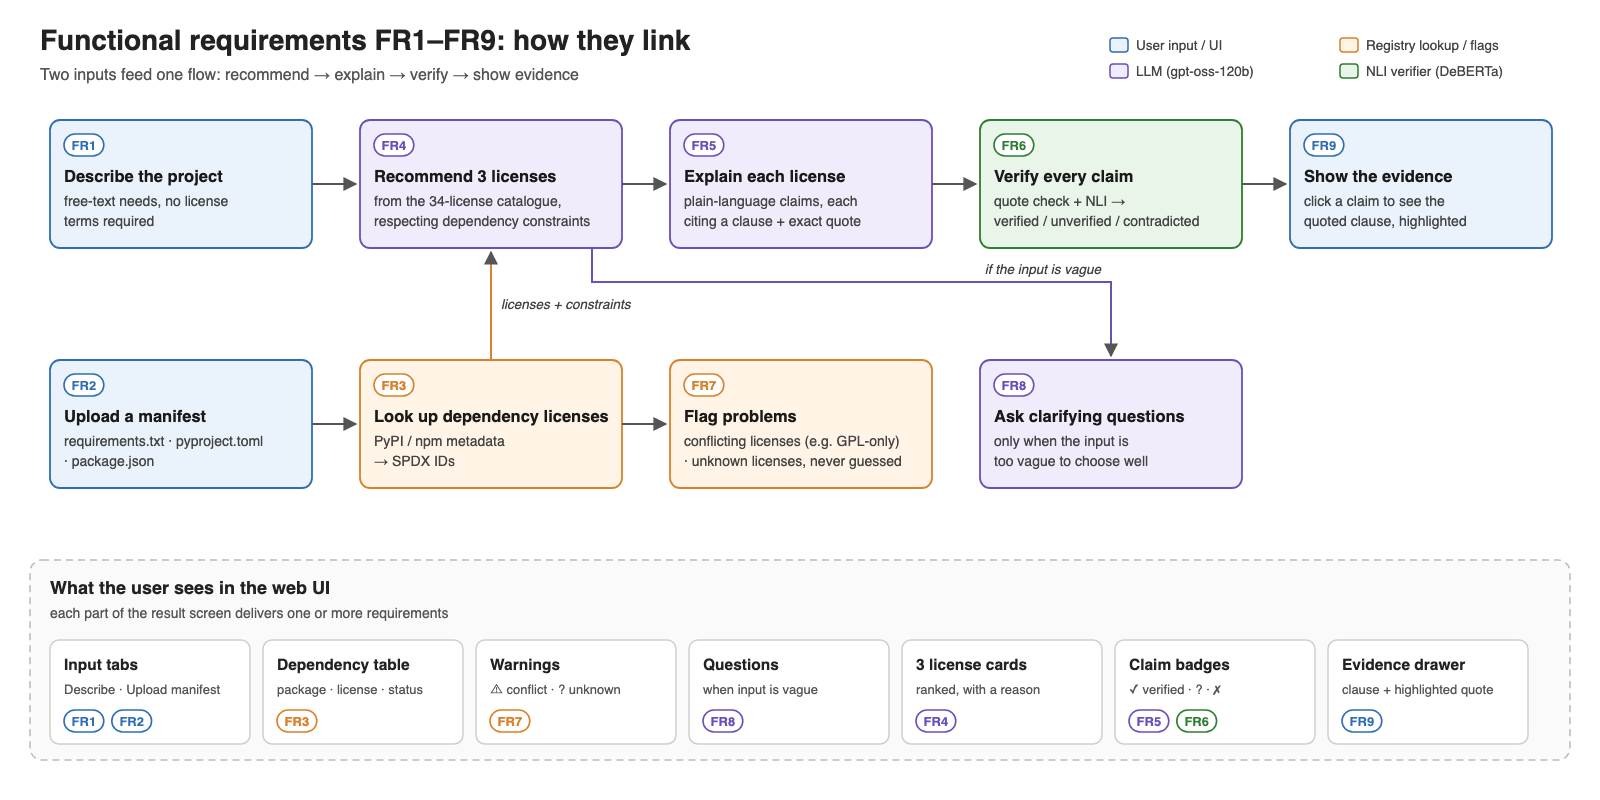
\includegraphics[width=0.92\textwidth]{13_functional_requirements.png}
    \caption{Functional requirements FR1--FR9 and how they link: two inputs feed one flow (recommend, explain, verify, show evidence); the bottom strip shows where each requirement appears in the user interface.}
    \label{fig:fr}
\end{figure*}

\paragraph{Architecture.}
Figure~\ref{fig:arch} shows the architecture. A React web UI sends requests to a FastAPI backend that runs the \texttt{licensewise} pipeline as a background job, because a request takes one to five minutes on the free API tier; the UI polls for the result. The pipeline has seven steps: (1) input validation; (2) dependency license lookup from PyPI or npm metadata, normalised to SPDX identifiers, with unrecognised licenses flagged as \emph{unknown} rather than guessed; (3) Stage~1, in which the LLM infers the developer's requirements and recommends exactly three licenses from the catalogue; (4) clause retrieval, which selects only the clauses of each license that express its obligations; (5) Stage~2, in which the LLM writes three to five claims per license, each citing one clause and quoting it verbatim; (6) NLI verification; and (7) response building. Offline components build the knowledge base and run the evaluation harness, which calls the same pipeline in batch.

\begin{figure*}[tb]
    \centering
    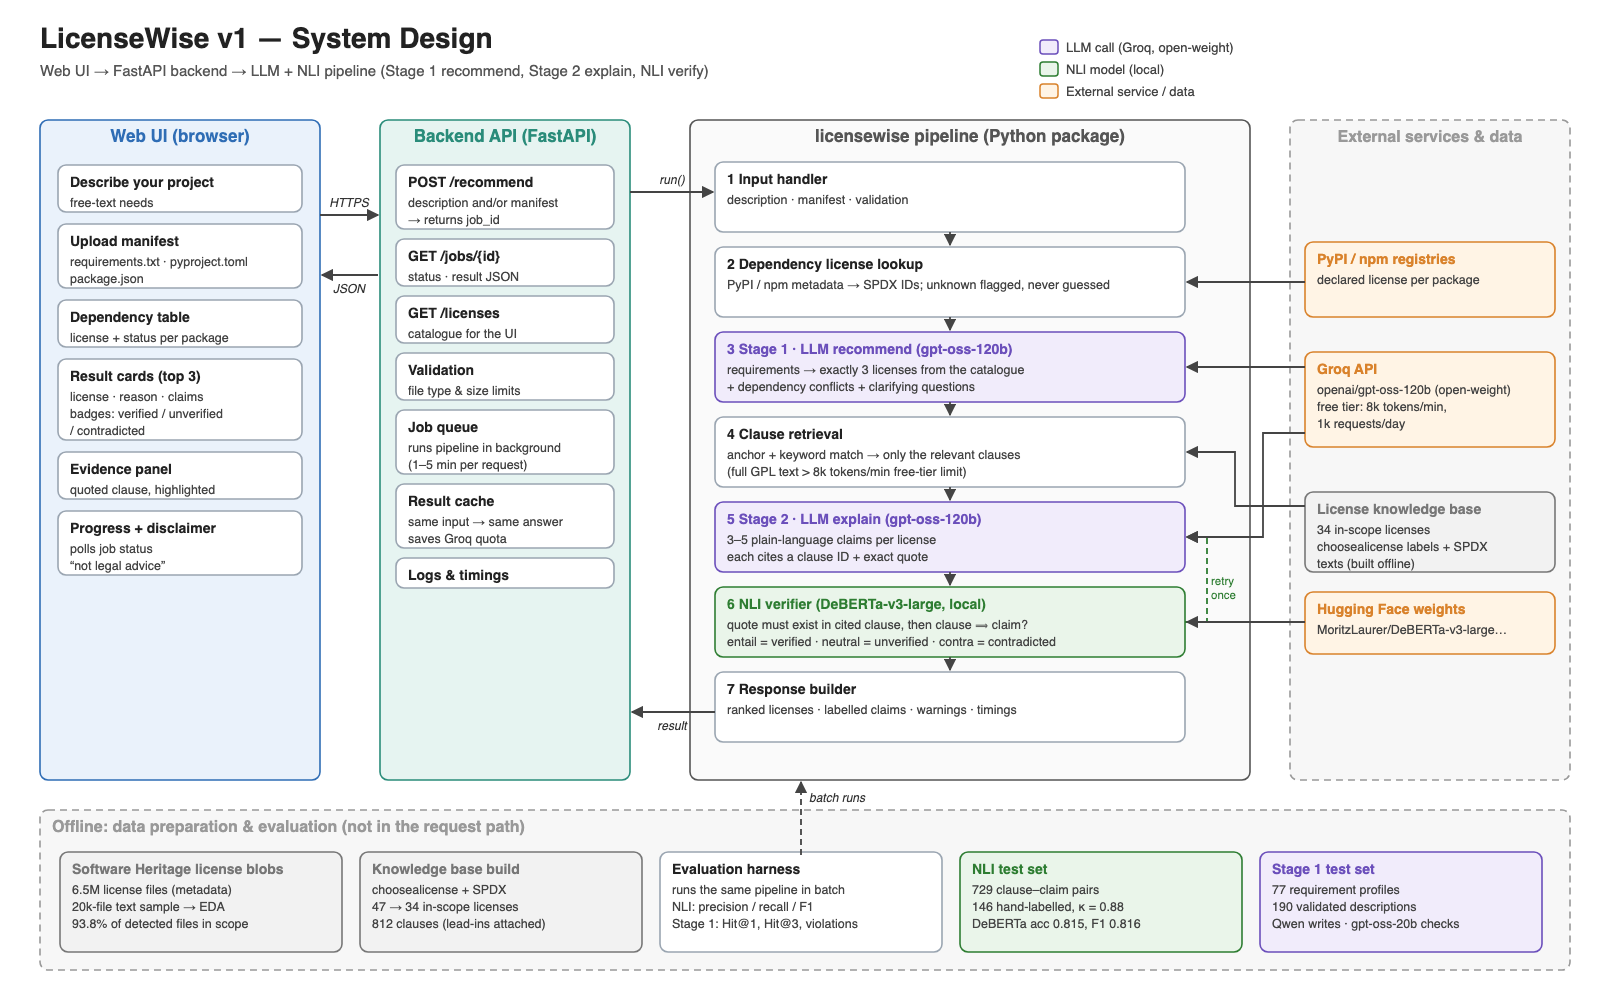
\includegraphics[width=\textwidth]{system_design.png}
    \caption{System design: web UI, FastAPI backend, and the seven-step LLM\,+\,NLI pipeline, with external services and the offline data-preparation and evaluation components.}
    \label{fig:arch}
\end{figure*}

\paragraph{User interface.}
Figure~\ref{fig:ui} shows the four-step user flow in the web interface: the developer describes the project (or uploads a manifest), the pipeline panel shows each step as it completes, the results show three license cards whose claims carry status badges, and selecting a claim opens the cited clause with the quoted words highlighted, together with the verifier's probabilities. Status badges always combine an icon with a text label, so status is never conveyed by colour alone. The UI is complete but not yet connected to the backend; it currently displays saved outputs of the real pipeline.

\begin{figure*}[tb]
    \centering
    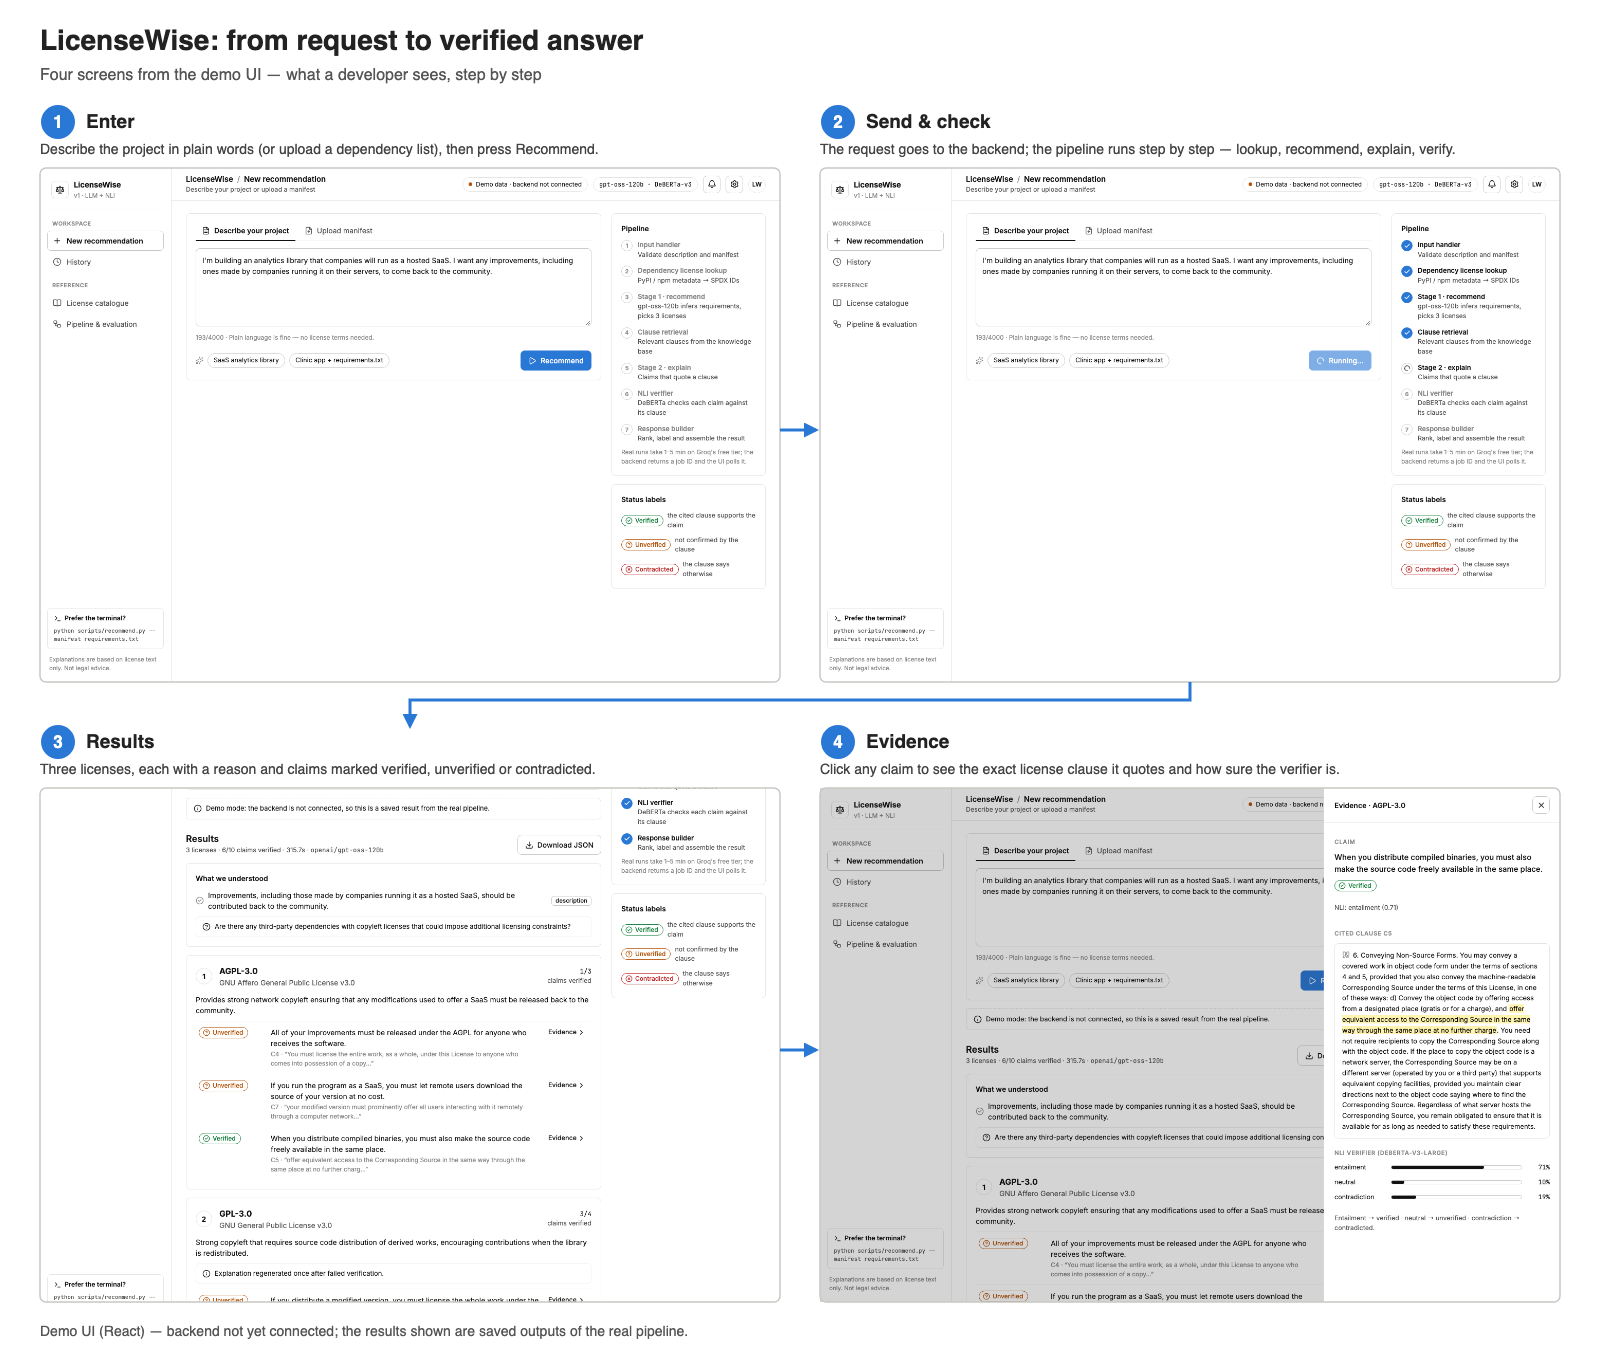
\includegraphics[width=0.92\textwidth]{22_ui_storyboard.png}
    \caption{User interface flow: (1) enter a description or manifest, (2) the pipeline runs, (3) results with verified/unverified/contradicted claims, (4) evidence drawer with the highlighted clause and NLI probabilities.}
    \label{fig:ui}
\end{figure*}

\paragraph{Implementation.}
The pipeline is a Python package (\texttt{licensewise}) with one module per step. All LLM calls request output that conforms to a JSON schema defined with Pydantic; the Stage~1 schema restricts license identifiers to the 34 catalogue entries and requires exactly three recommendations, and a duplicate recommendation triggers one retry. Stage~2 is re-run once, with the failed claims listed, if more than half of a license's claims fail verification. The web UI is built with React, TypeScript, and Vite. Data preparation and evaluation are reproducible scripts, and a Jupyter notebook reproduces every figure and result in this report.

\subsection{Machine Learning}
\label{ss:ml}

\begin{table}[tb]
    \caption{Models used in Phase 1. No model was fine-tuned.}
    \label{tab:models}
    \small
    \begin{tabularx}{\columnwidth}{@{}p{2.3cm}X@{}}
        \toprule
        \textbf{Model} & \textbf{Role and rationale} \\
        \midrule
        gpt-oss-120b (open-weight, via Groq~\cite{groq}) & Stage~1 recommendation and Stage~2 explanation. Maps informal intent to license concepts; strict JSON-schema output; free tier. \\
        DeBERTa-v3-large NLI~\cite{he2023debertav3,laurer2024less} & Verifier. Pre-trained by its authors on MNLI, FEVER-NLI, ANLI, LingNLI, and WANLI; used as-is, locally. Independent of the LLM. \\
        RoBERTa-large-MNLI~\cite{liu2019roberta} & Baseline verifier for RQ2. \\
        Qwen3.8-27B (via Groq) & Writes test descriptions (evaluation only). \\
        gpt-oss-20b (via Groq) & Checks test descriptions blind (evaluation only). \\
        \bottomrule
    \end{tabularx}
\end{table}

Table~\ref{tab:models} lists the models. The recommender and explainer use \textbf{gpt-oss-120b}, an open-weight model served through the Groq API. It is used \emph{zero-shot}: it receives instructions and the license catalogue but no examples and no task-specific training. An LLM is needed because translating informal preferences into license concepts such as copyleft or network-use clauses requires language understanding that fixed rules cannot provide.

The verifier is \textbf{DeBERTa-v3-large} fine-tuned for NLI by its authors on several public corpora~\cite{laurer2024less}; we did not train it. For each claim, the cited clause is the \emph{premise} and the claim is the \emph{hypothesis}; the model outputs probabilities for entailment, neutral, and contradiction, and the highest becomes the user-facing status (verified, unverified, contradicted). Before the NLI call, a quote check confirms that the quoted text appears verbatim in the cited clause; if not, the claim is marked unverified. An independent verifier is valuable because it does not share the LLM's errors, and its outputs double as an automatic faithfulness measure. We selected DeBERTa over a RoBERTa-large-MNLI baseline on the basis of RQ2 (Section~\ref{ss:rq2}).

Two further models are used only to build test data: Qwen3.8-27B writes project descriptions and gpt-oss-20b validates them. Using different models from the one under test reduces the risk that the system is evaluated on its own phrasing.

\subsection{Changes Since the Proposal}
\label{ss:changes}

The proposal described a fuller neuro-symbolic design with a rules engine, retrieval over a vector store, repository scanning, and fine-tuned models, with a hosted commercial LLM and validation by domain experts. Phase~1 deliberately implements a smaller core (v1) that can be built and evaluated end to end: an open-weight LLM via a free API instead of a hosted commercial model; selection of relevant clauses by keyword matching instead of vector retrieval, because full license texts exceed the free tier's per-minute token limit; registry metadata instead of repository scanning; no fine-tuning; and expert-free ground truth from curated public data. The rules engine and compatibility matrix are deferred to Phase~2, and the results below indicate that they are needed.

\section{Methodology}
\label{s:method}

\subsection{Data Sources}
\label{ss:data}

\paragraph{choosealicense.com.} The repository behind choosealicense.com~\cite{choosealicense} contains 47 license files, each with a YAML header and the full license text. We keep the SPDX identifier, title, description, the three label lists, and the text, and drop website-only fields (installation instructions, example projects, display flags). The label vocabulary has 5 permissions (commercial use, modifications, distribution, private use, patent use), 8 conditions (include copyright, include copyright in source, document changes, disclose source, same license, same license for files, same license for libraries, network use is distribution), and 4 limitations (liability, warranty, trademark use, patent use). These labels are the facts from which all our ground truth is computed.

\paragraph{SPDX license list.} From the SPDX list (v3.29.0, 740 identifiers)~\cite{spdx} we keep each identifier and its OSI-approval flag, used to scope the catalogue and to normalise dependency licenses.

\paragraph{Software Heritage license dataset.} This dataset~\cite{zacchiroli2022dataset} describes 6.5 million deduplicated license files from public software origins. We use five metadata tables (file names and identifiers, file information, ScanCode license detections, first appearance and popularity, example origin) and the published 20{,}000-file random text sample; we do not download the 14\,GB full-text archive. The sample is joined to the five tables on two keys (SHA1 content hash and Software Heritage identifier), producing a 20{,}000-row table with 16 columns. It is used for exploratory analysis and to measure scope coverage, not as ground truth.

\paragraph{Package registries.} At run time, dependency licenses are read from PyPI (\texttt{license\_expression}, \texttt{license}, then trove classifiers) and npm (\texttt{license}), and normalised to SPDX identifiers with exact matching and 41 common spellings. Development-only dependencies are ignored because they are not shipped.

\subsection{Scope and Preprocessing}
\label{ss:prep}

We remove licenses not intended for software (8: media, documentation, data, fonts, and hardware licenses) and licenses not approved by the OSI (5), leaving \textbf{34 in-scope licenses}. A language check (share of common French words per paragraph) identifies CeCILL-2.1 as French-only; it remains recommendable, but its claims cannot be verified by the English-only verifier. Each license is classed as permissive (21), weak copyleft (4), or strong copyleft (9) directly from its labels.

\paragraph{Clause segmentation.} The verifier accepts at most 512 tokens, while GPL-3.0 alone is about 35{,}000 characters; claims must also be checked against the one passage that supports them, and users need a specific passage as evidence. We therefore split each license into clauses: split at blank lines, drop non-English paragraphs, merge short headings into the following paragraph, and attach a paragraph ending in a colon (a lead-in) to each list item below it, so that no clause stops at ``\ldots to do the following:'' (Figure~\ref{fig:clauses}). This yields \textbf{812 clauses} from 33 English licenses (median 329 characters; all within the verifier's input limit).

\begin{figure}[tb]
    \centering
    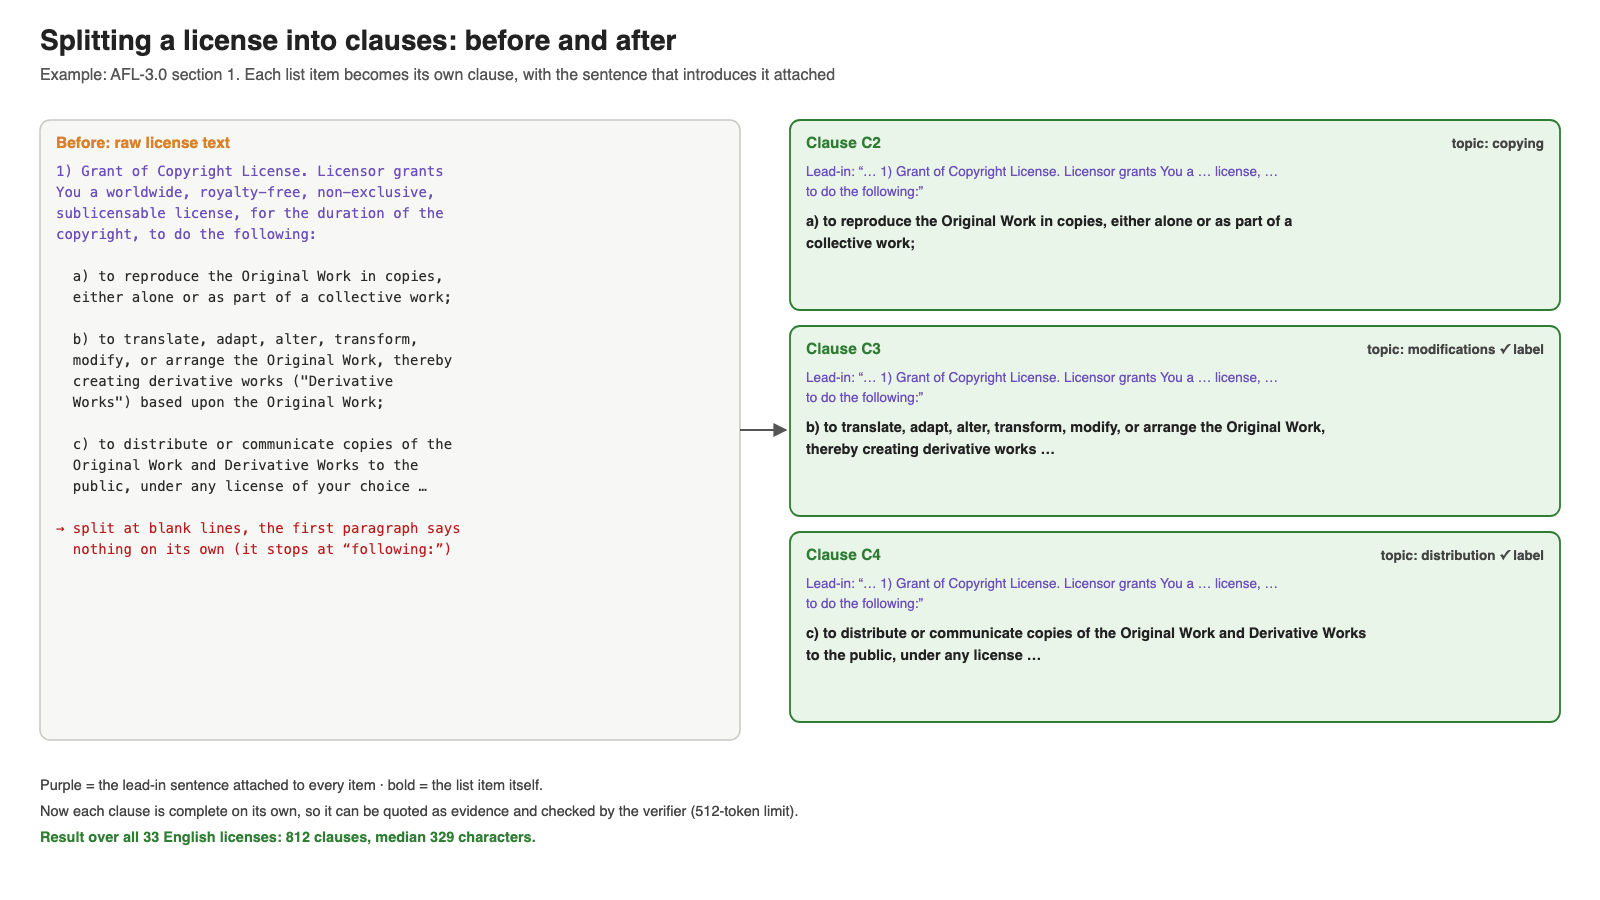
\includegraphics[width=\columnwidth]{25_clause_split.png}
    \caption{Clause segmentation on AFL-3.0: each list item becomes a clause with its lead-in sentence attached.}
    \label{fig:clauses}
\end{figure}

\paragraph{Finding the clause for a label.} For each of 16 labels we define a precise anchor pattern (e.g., ``Limitation of Liability'', ``Grant of Patent License'') and a broader keyword pattern. Clauses are ranked by anchor matches, then keyword matches, then position. We checked the selections by hand on MIT, BSD, Apache-2.0, GPL-3.0, and MPL-2.0. The same procedure selects evidence clauses for Stage~2 at run time.

\subsection{Ground Truth for RQ1: Profiles and Descriptions}
\label{ss:gt1}

No public dataset pairs developer requests with known correct licenses, so we construct one in which the answers are computed rather than judged.

\paragraph{Requirement profiles.} From the 17 labels we keep those that differ between in-scope licenses and that a developer would state as a need, giving six requirements: share changes (none, file/library level, whole work), network use (must trigger sharing, must not), patent grant, trademark protection, no attribution required, and no obligation to document changes. Labels held by every license (e.g., commercial use, warranty disclaimer) or by none are excluded because they cannot distinguish licenses. Allowing ``don't care'' for each requirement gives $4 \times 3 \times 2 \times 2 \times 2 \times 2 = 192$ combinations, or 191 excluding the empty request. For each combination, the \emph{answer key} is the set of in-scope licenses whose labels satisfy every requirement. 114 combinations have no satisfying license and are discarded, leaving \textbf{77 profiles} with 1 to 29 correct licenses each (median 3).

\paragraph{Natural-language descriptions.} Real developers describe projects in their own words rather than as requirement lists, and with structured requirements a simple label lookup, the same one that builds the answer key, would make an LLM unnecessary. We therefore test the recommender on natural-language descriptions. Qwen3.8-27B writes about three first-person descriptions per profile, each from a different persona and project type and never naming a license; persona variety tests whether the system understands meaning rather than one phrasing. gpt-oss-20b then reads each description \emph{without} the profile and lists the requirements it can identify; a description is kept only if they match the profile exactly. Of 235 descriptions written, \textbf{190} (81\%) pass, covering 70 of the 77 profiles. The writer produced 122 distinct persona labels, most often ``startup founder'' (29) and ``university researcher'' (25).

\subsection{Ground Truth for RQ2: Clause--Claim Pairs}
\label{ss:gt2}

For each English license and each label it carries, we take the clause selected for that label and build three pairs from 16 claim templates (one true and one negated sentence per label; private use is excluded because no license states it in a single clause): the true claim (\emph{entailment}), the negated claim (\emph{contradiction}), and a true claim about another label whose keywords do not appear in the clause (\emph{neutral}). Of 266 license--label combinations, 23 have no matching clause (mostly commercial use, as licenses such as BSD never mention selling), leaving 243 and therefore \textbf{729 pairs} (243 per label) built on 173 distinct clauses. The claims and labels are written by templates, not by any model; the NLI model only predicts labels for evaluation.

\paragraph{Human validation.} Because the labels are automatic, two annotators checked a stratified random sample of 150 pairs (50 per label): the first author, and a software engineer with experience working with open-source licenses who is now a software engineering researcher. Each labelled 75 pairs, judging only from the given clause. Disagreements with the automatic labels (22) were settled by the team; 3 remained ambiguous and were excluded, leaving \textbf{146 labelled pairs}. A later fix to clause segmentation changed 23 sampled pairs, which were relabelled. To measure inter-annotator agreement, each annotator also labelled 20 of the other's pairs.

\subsection{Evaluation Protocol and Metrics}
\label{ss:metrics}

\paragraph{RQ1.} Stage~1 (gpt-oss-120b) receives only the description text and the catalogue. For each description we compute Hit@1 (the first recommendation is in the answer key), Hit@3 (at least one of the three is), and Precision@3 (the share of the three that are), and for each requirement the share of recommendations that violate it. Results are grouped by the size of the answer key (1--3, 4--10, more than 10 correct licenses) as a measure of request specificity. Groq's free tier limits gpt-oss-120b to 200{,}000 tokens per day, so we evaluated one description per profile first and stopped at \textbf{104 descriptions covering all 70 profiles}.

\paragraph{RQ2.} DeBERTa-v3-large and RoBERTa-large-MNLI are run on all 729 pairs (premise = clause, hypothesis = claim). We report accuracy, per-class precision, recall, and F1, and macro-F1, against the automatic labels and against the 146 human labels. The key metric is \emph{entailment precision}: how often a \emph{verified} status is correct. Agreement is measured with Cohen's $\kappa$~\cite{cohen1960kappa}.

\paragraph{RQ3.} For complete pipeline runs we measure the share of quotes found verbatim in their cited clause and the distribution of verified, unverified, and contradicted claims. In Phase~1 this is limited to two end-to-end runs; the comparison with an unverified (LLM-only) baseline is planned for Phase~2.

\section{Results}
\label{s:results}

\subsection{Exploratory Analysis}
\label{ss:eda}

In the 20{,}000-file Software Heritage sample, 52\% of files contain exactly one in-scope license detected with full confidence, 6\% a likely modified (variant) license, and 8\% several licenses; 4\% contain only out-of-scope licenses and 28\% contain no license at all (mostly \texttt{AUTHORS} files and HTML pages). Of the files with any detected license, \textbf{93.8\%} use one of our 34 licenses, which supports the chosen scope. Usage is highly skewed (Figure~\ref{fig:toplic}): MIT accounts for 70.5\% of in-scope files, followed by BSD-3-Clause (6.9\%), Apache-2.0 (6.2\%), GPL-2.0 (4.6\%), and GPL-3.0 (4.1\%), across 488 distinct license identifiers. ScanCode confidence is high (mean 99.1; 87.9\% of detections at 100). The median license file has 169 words, and 76\% of files first appeared in public history in 2015 or later. In the knowledge base, the most common conditions are include copyright (29 of 34 licenses), disclose source (14), and document changes (14); only five licenses have a network-use clause.

\begin{figure}[tb]
    \centering
    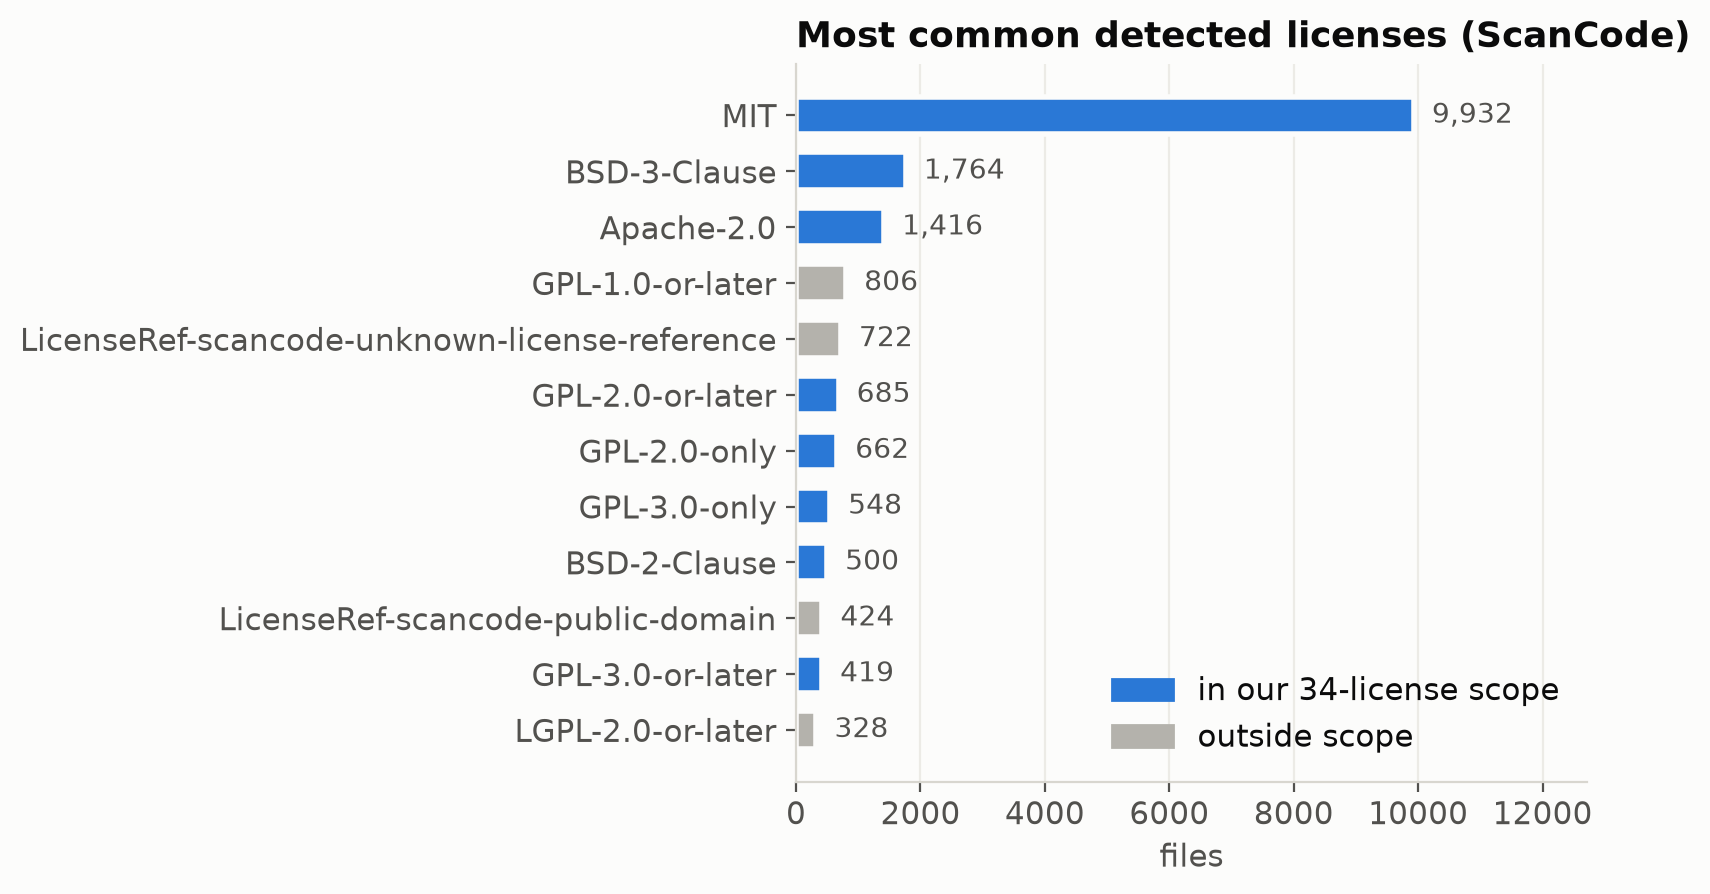
\includegraphics[width=\columnwidth]{02_top_licenses.png}
    \caption{Most common detected licenses in the Software Heritage sample (blue: in our scope).}
    \label{fig:toplic}
\end{figure}

\subsection{RQ1: Requirement-to-License Mapping}
\label{ss:rq1}

\begin{table}[tb]
    \caption{Stage 1 (gpt-oss-120b) on 104 descriptions, grouped by the number of correct licenses (answer-key size).}
    \label{tab:rq1}
    \small
    \begin{tabular}{@{}lrrrr@{}}
        \toprule
        \textbf{Correct licenses} & \textbf{n} & \textbf{Hit@1} & \textbf{Hit@3} & \textbf{Prec@3} \\
        \midrule
        1--3 (hardest) & 47 & 0.40 & 0.60 & 0.42 \\
        4--10 & 35 & 0.54 & 0.77 & 0.51 \\
        $>$10 (easiest) & 22 & 0.91 & 1.00 & 0.88 \\
        \midrule
        \textbf{All} & \textbf{104} & \textbf{0.56} & \textbf{0.74} & \textbf{0.55} \\
        \bottomrule
    \end{tabular}
\end{table}

Table~\ref{tab:rq1} and Figure~\ref{fig:rq1} summarise RQ1. Overall, the first recommendation is correct for 56\% of descriptions and a correct license appears in the top three for 74\%. Accuracy depends strongly on specificity: for broad requests (more than ten correct licenses) the model is nearly perfect (Hit@3 = 1.00), but when only one to three licenses satisfy the requirements, a correct license appears in the top three for only 60\% of descriptions and the first pick is correct for only 40\%.

Requirement violations (Figure~\ref{fig:viol}) show where recommendations go wrong. Trademark protection is the requirement most often broken (54\% of recommendations for profiles that require it), followed by ``no obligation to document changes'' (39\%), the level of copyleft (21\%), and the network-use clause (12\%); patent grant is rarely violated (4\%) and attribution never. The model also over-relies on Apache-2.0, its first choice for 30 of 104 descriptions, including cases where Apache-2.0's requirement to mark changed files violates a stated need.

\begin{figure}[tb]
    \centering
    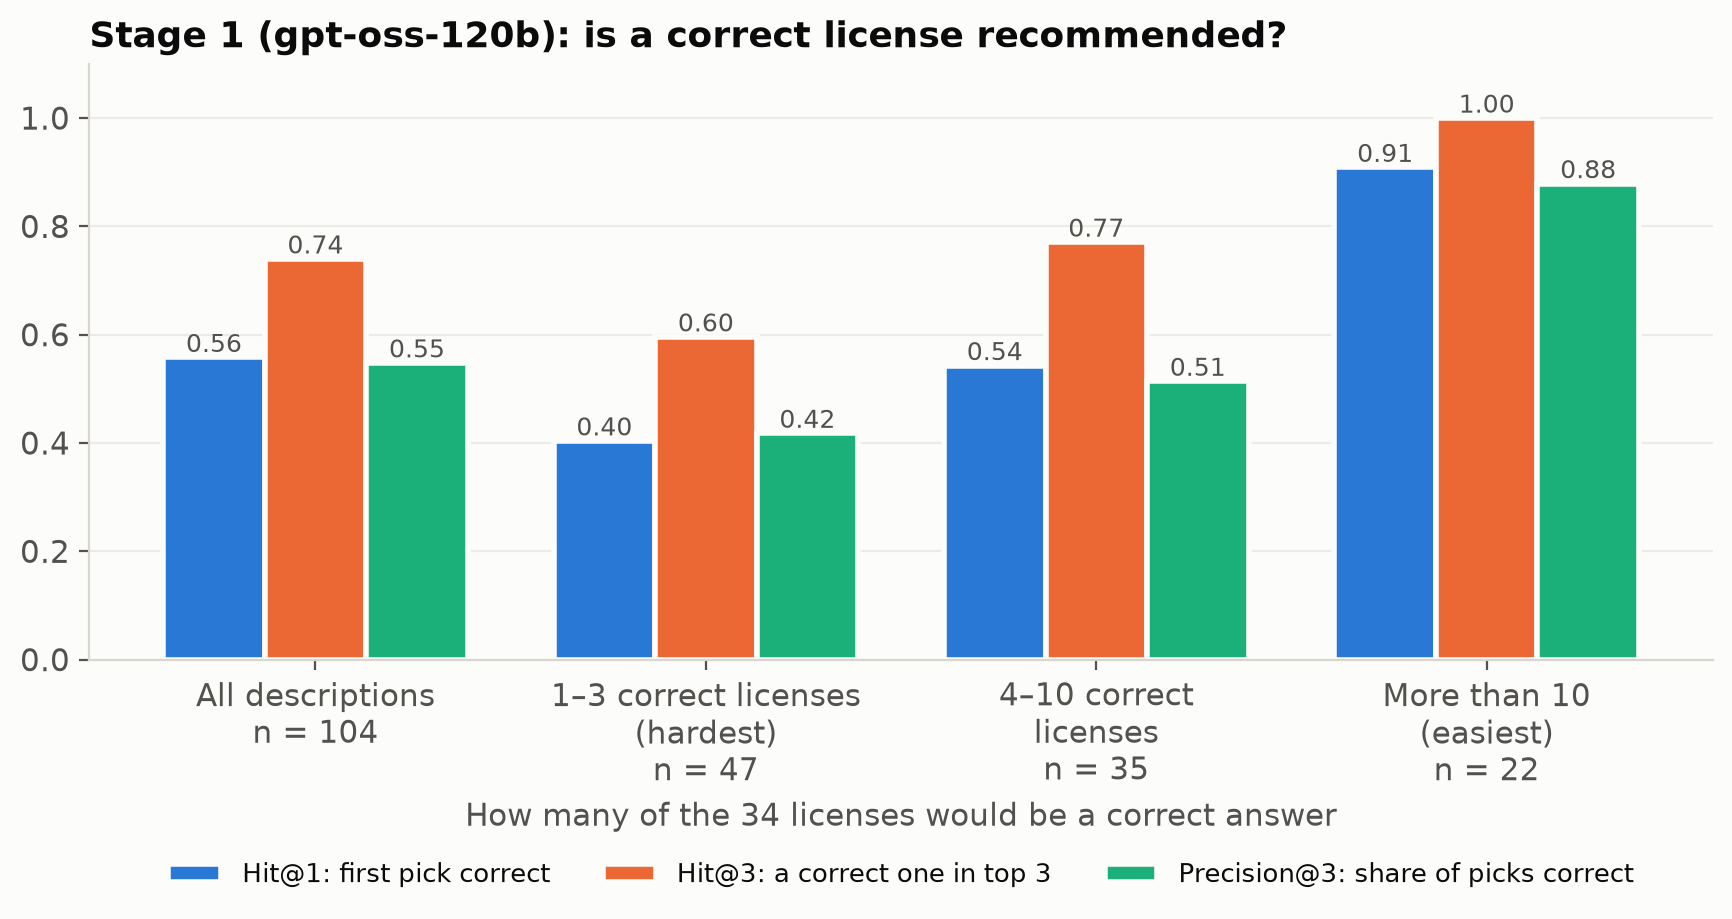
\includegraphics[width=\columnwidth]{10_stage1_hits.png}
    \caption{RQ1: Hit@1, Hit@3, and Precision@3 by answer-key size.}
    \label{fig:rq1}
\end{figure}

\begin{figure}[tb]
    \centering
    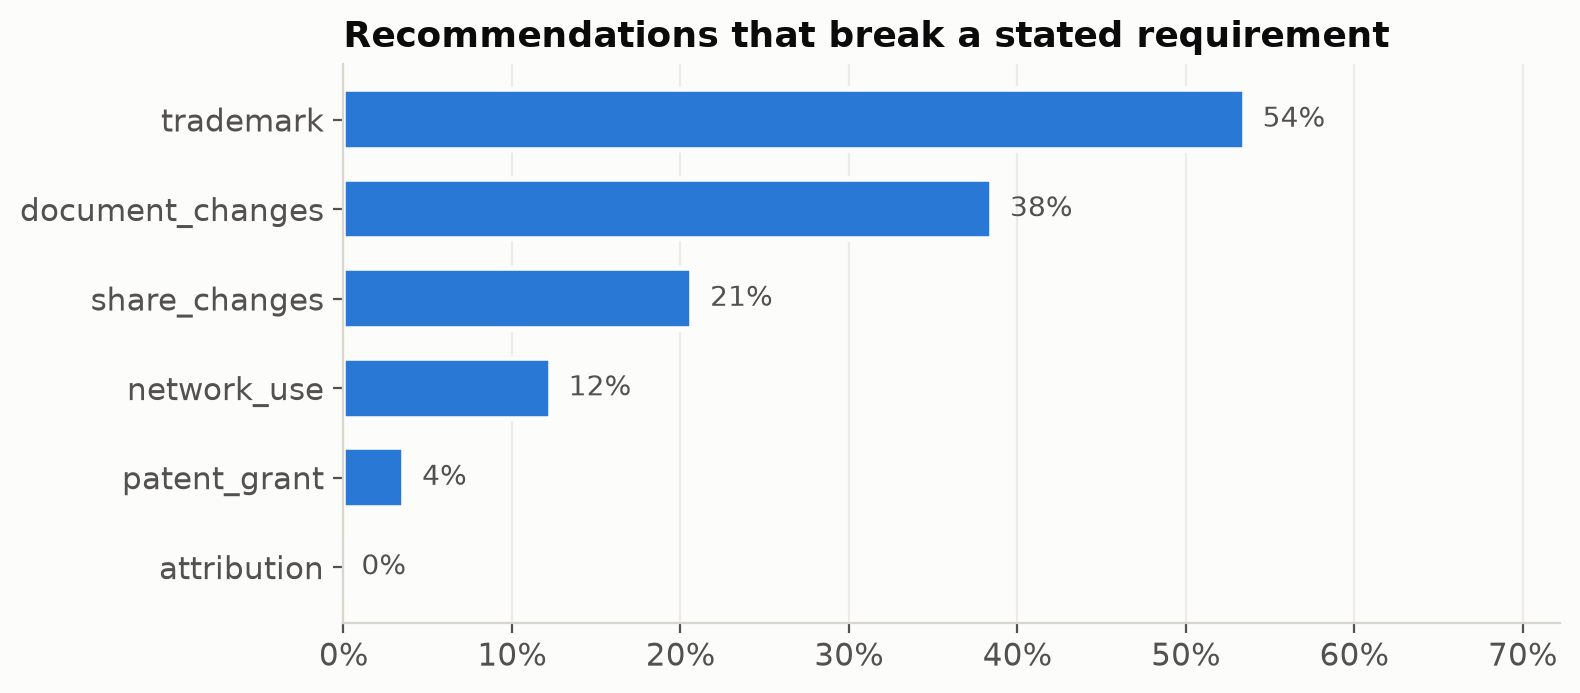
\includegraphics[width=\columnwidth]{11_stage1_violations.png}
    \caption{RQ1: share of recommendations that violate each stated requirement.}
    \label{fig:viol}
\end{figure}

\subsection{RQ2: Claim Verification}
\label{ss:rq2}

\paragraph{Label quality and agreement.} The automatic labels agree with the final human labels on 143 of 146 pairs (\textbf{97.9\%}), so the full 729-pair set can be used with confidence. On the 39 pairs labelled by both annotators, agreement is 92.3\% with Cohen's $\kappa = 0.88$, ``almost perfect'' on the Landis and Koch scale~\cite{landis1977agreement}; the second annotator could see the first label, which may inflate this value.

\begin{table}[tb]
    \caption{NLI verifiers on 146 human-labelled pairs (P/R/F1 per class).}
    \label{tab:rq2}
    \small
    \begin{tabular}{@{}llrrr@{}}
        \toprule
        \textbf{Model} & \textbf{Class} & \textbf{P} & \textbf{R} & \textbf{F1} \\
        \midrule
        \multirow{3}{*}{RoBERTa-large} & entailment & 0.900 & 0.551 & 0.684 \\
                                       & neutral & 0.583 & 0.745 & 0.654 \\
                                       & contradiction & 0.804 & 0.900 & 0.849 \\
        \multicolumn{2}{@{}l}{\quad accuracy 0.733; macro-F1 0.729} & & & \\
        \midrule
        \multirow{3}{*}{DeBERTa-v3-large} & entailment & \textbf{0.944} & \textbf{0.694} & \textbf{0.800} \\
                                          & neutral & 0.672 & 0.872 & 0.759 \\
                                          & contradiction & 0.898 & 0.880 & 0.889 \\
        \multicolumn{2}{@{}l}{\quad accuracy \textbf{0.815}; macro-F1 \textbf{0.816}} & & & \\
        \bottomrule
    \end{tabular}
\end{table}

\paragraph{Model comparison.} Table~\ref{tab:rq2} reports both verifiers on the human-labelled pairs. DeBERTa-v3-large outperforms RoBERTa-large-MNLI on every class, with accuracy 0.815 versus 0.733 and macro-F1 0.816 versus 0.729. On all 729 automatically labelled pairs the ranking is the same (accuracy 0.809 versus 0.782). We therefore use DeBERTa as the verifier.

\begin{table}[tb]
    \caption{DeBERTa confusion matrix on 146 human-labelled pairs (rows: human label; columns: prediction).}
    \label{tab:cm}
    \small
    \begin{tabular}{@{}lrrr@{}}
        \toprule
        & \textbf{entail.} & \textbf{neutral} & \textbf{contrad.} \\
        \midrule
        entailment & \textbf{34} & 14 & 1 \\
        neutral & 2 & \textbf{41} & 4 \\
        contradiction & 0 & 6 & \textbf{44} \\
        \bottomrule
    \end{tabular}
\end{table}

\paragraph{Error profile.} The confusion matrix (Table~\ref{tab:cm}) shows that the verifier errs on the side of caution. When it predicts entailment (shown to users as \emph{verified}) it is correct 94\% of the time, and it never labelled a false (contradicted) claim as entailed. Its main weakness is recall on true claims: 14 of 49 entailed claims (29\%) were judged neutral and would appear as \emph{unverified}. Six contradictions were also judged neutral, and four neutral claims were wrongly flagged as contradictions. Figure~\ref{fig:recall} breaks entailment recall down by label: claims about document changes (91\%), liability (90\%), and distribution (84\%) are usually confirmed, whereas claims about commercial use (21\%), same-license copyleft (25\%), and network use (25\%) rarely are. These are the labels for which a license states the obligation in different terms from the claim; for example, a license says ``sell'' or ``charge a fee'' rather than ``commercial use''.

\begin{figure}[tb]
    \centering
    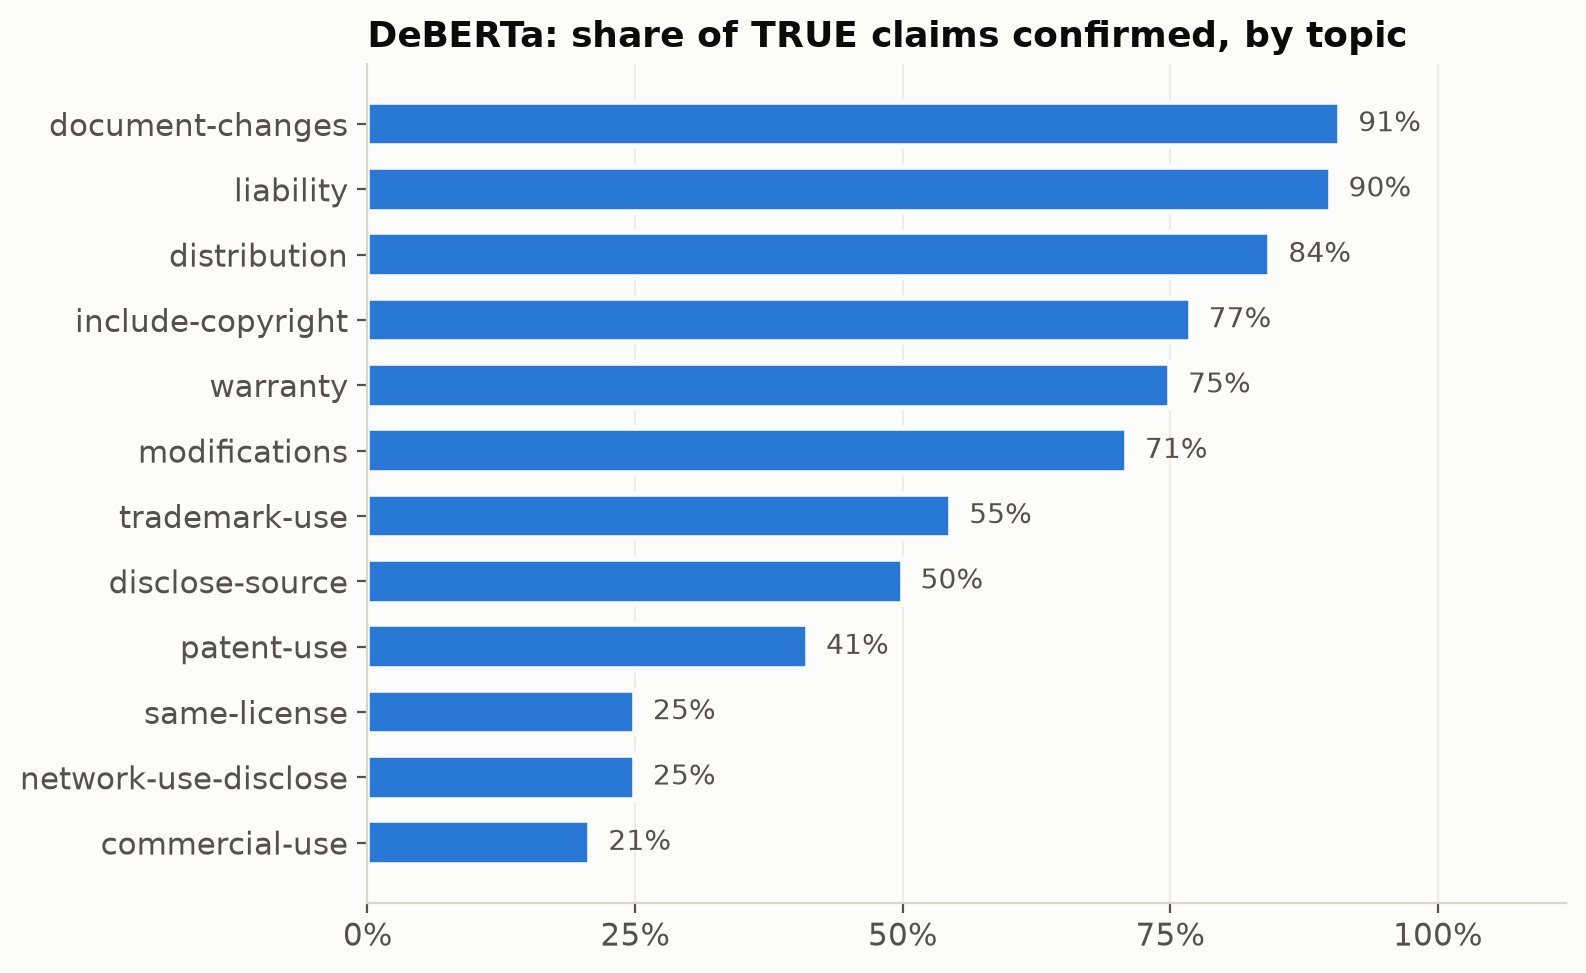
\includegraphics[width=\columnwidth]{09_nli_recall_by_label.png}
    \caption{RQ2: share of true claims confirmed by DeBERTa, by license label (729 automatically labelled pairs).}
    \label{fig:recall}
\end{figure}

\subsection{RQ3: Explanation Faithfulness (Preliminary)}
\label{ss:rq3}

Two complete pipeline runs produced 19 claims across six license recommendations. All 19 quotes (100\%) were found verbatim in their cited clauses, indicating that clause-level grounding constrains the explainer's quotations. Of the claims, 11 (58\%) were verified, 7 (37\%) unverified, and 1 (5\%) contradicted. Manual inspection of the unverified claims shows that most were correct statements of copyleft or commercial-use terms, consistent with the RQ2 error profile, and the single contradicted claim (an accurate paraphrase of AGPL-3.0 section~6) was a verifier false positive. A systematic comparison with an unverified baseline is left to Phase~2.

\section{Discussion}
\label{s:discussion}

\paragraph{LLMs interpret intent well but should not decide license facts alone.}
RQ1 shows a clear pattern: the recommender handles broad requests almost perfectly but degrades as requests become specific, exactly where developers most need help. The errors are not random: a few requirements (trademark protection, change documentation, copyleft level) account for most violations, and the model gravitates towards popular licenses such as Apache-2.0. Because these are factual properties already encoded in the license labels, a deterministic step can check them. This supports the neuro-symbolic design planned for Phase~2: the LLM converts the description into structured requirements, and a rule engine over the labels (and the OSADL compatibility matrix for dependencies) selects the licenses. The LLM then does what it does well, interpreting language, and the lookup, which cannot misstate a license's labels, does the matching. An ``oracle-input'' experiment, giving Stage~1 the exact requirements instead of the description, would separate misunderstanding errors from license-knowledge errors and indicate how much of the gap such a design can close.

\paragraph{An off-the-shelf verifier is cautious, which suits this domain.}
RQ2 shows that DeBERTa rarely confirms a claim that is not supported (precision 0.94), and it never confirmed a false claim in the human-labelled set. In licensing, the cost of a wrong ``verified'' is higher than the cost of a missing one, so this error profile is acceptable for a first version, provided that the interface presents ``unverified'' as ``not confirmed by the clause'' rather than ``wrong''. The verifier's weakness is concentrated in claims that require a small inferential step beyond the clause wording (``sell'' $\rightarrow$ commercial use; ``license the entire work under this License'' $\rightarrow$ same-license copyleft). Two remedies follow: prompting the explainer to phrase claims in the license's own vocabulary, which our clause-cited design already encourages, and fine-tuning the verifier on license-domain pairs such as ours, split by license to avoid leakage.

\paragraph{Grounding makes explanations checkable.}
Requiring each claim to cite and quote a specific clause made every explanation in our runs traceable: all quotes were verbatim, and each claim can be inspected by the user in one click. Even when the verifier is uncertain, the user can read the evidence directly, which is the transparency property we prioritised.

\paragraph{Expert-free evaluation is feasible with care.}
Computing answer keys from curated labels, generating test inputs with one model and validating them with another, and checking automatic labels with a small human sample gave us evaluation data whose quality we could measure (97.9\% label accuracy; $\kappa = 0.88$). The approach transfers to other domains where curated structured data exists but expert annotators do not.

\section{Limitations and Threats to Validity}
\label{s:limits}

\paragraph{Construct validity.}
Our ground truth is the choosealicense.com label set. Labels are a simplification of legal text, and some are debatable; for example, both EPL versions are labelled \emph{same license}, although EPL is often described as weak copyleft. The six requirements were chosen by us from the labels rather than elicited from developers, and the tool explains license \emph{text}, not legal interpretation or case law.

\paragraph{Internal validity.}
The test descriptions are written by an LLM and validated by another LLM. They may be cleaner and more explicit than real requests, and the round-trip filter keeps only clearly expressible requirements, so weak copyleft and ``network use must not trigger sharing'' are under-represented (7 profiles have no valid description). The writer occasionally returned more or fewer than three descriptions per profile (235 rather than 231), although each profile was evaluated once first. NLI labels are automatic; we measured their accuracy on a 146-pair sample, but in the agreement check the second label was assigned with the first visible, which may inflate $\kappa$. One clause-segmentation defect remains: in AFL-3.0 and OSL-3.0, numbered sections after section~1 are treated as list items of section~1's lead-in, so those clauses begin with an irrelevant sentence.

\paragraph{External validity.}
The catalogue contains only OSI-approved software licenses, the verifier is English-only (CeCILL-2.1 cannot be verified), and dual licensing (e.g., commercial licenses offered alongside the GPL) is out of scope. Results are for one LLM and two NLI models; other models may behave differently.

\paragraph{Reliability and scale.}
Due to the free API tier (200{,}000 tokens per day for gpt-oss-120b), RQ1 covers 104 of 190 valid descriptions (all 70 profiles, at least once each), and RQ3 is based on two end-to-end runs. LLM outputs are non-deterministic; we did not repeat runs to measure variance. The web UI is not yet connected to the backend, and a request takes one to five minutes on the free tier.

\section{Conclusion and Future Work}
\label{s:conclusion}

We presented \sys{}, an LLM\,+\,NLI pipeline that recommends open-source licenses and explains them with clause-cited claims, each checked by an independent verifier. Using evaluation data built entirely from public, curated sources, we found that an open-weight LLM places a correct license in its top three for 74\% of developer descriptions, but only 60\% when few licenses fit; and that an off-the-shelf NLI verifier is reliable when it confirms a claim (precision 0.94) but leaves about three in ten true claims unconfirmed. Explanations were fully traceable to verbatim license text.

Phase~2 will (1) add a rule engine that selects licenses from structured requirements and checks dependency compatibility against the OSADL matrix; (2) connect the web UI to the FastAPI backend with job queuing, caching, and operational warnings; (3) complete RQ3 with a verified-versus-unverified comparison over all descriptions; (4) run the oracle-input experiment; (5) improve the verifier through claim phrasing, threshold tuning, or license-domain fine-tuning, and fix the remaining clause-segmentation defect; and (6) conduct a small user study on the clarity and usefulness of the explanations.


\bibliographystyle{ACM-Reference-Format}
\bibliography{references}

\end{document}
